%%% Hlavní soubor. Zde se definují základní parametry a odkazuje se na ostatní části. %%%

%% Verze pro jednostranný tisk:
% Okraje: levý 40mm, pravý 25mm, horní a dolní 25mm
% (ale pozor, LaTeX si sám přidává 1in)
\documentclass[12pt,a4paper]{report}
\setlength\textwidth{145mm}
\setlength\textheight{247mm}
\setlength\oddsidemargin{15mm}
\setlength\evensidemargin{15mm}
\setlength\topmargin{0mm}
\setlength\headsep{0mm}
\setlength\headheight{0mm}
% \openright zařídí, aby následující text začínal na pravé straně knihy
\let\openright=\clearpage

%% Pokud tiskneme oboustranně:
% \documentclass[12pt,a4paper,twoside,openright]{report}
% \setlength\textwidth{145mm}
% \setlength\textheight{247mm}
% \setlength\oddsidemargin{15mm}
% \setlength\evensidemargin{0mm}
% \setlength\topmargin{0mm}
% \setlength\headsep{0mm}
% \setlength\headheight{0mm}
% \let\openright=\cleardoublepage

%% Použité kódování znaků: obvykle latin2, cp1250 nebo utf8:
\usepackage[utf8]{inputenc}
%% Ostatní balíčky
\usepackage{graphicx}
\usepackage{amsthm}
\usepackage[outdir=./]{epstopdf}
\usepackage[english]{babel}
\usepackage{blindtext}

%% Balíček hyperref, kterým jdou vyrábět klikací odkazy v PDF,
%% ale hlavně ho používáme k uložení metadat do PDF (včetně obsahu).
%% POZOR, nezapomeňte vyplnit jméno práce a autora.
\usepackage[unicode]{hyperref}   % Musí být za všemi ostatními balíčky
\hypersetup{pdftitle=Development of an English public transport information dialogue system}
\hypersetup{pdfauthor=Martin Vejman}


%% \todo{} command.
%
% Outputs red TODOs in the document. Requires \usepackage{color}.
%
% Usage: \todo{Document the TODO command.}
%
% Comment out second line to disable.
\usepackage{color}
\newcommand{\todo}[1]{}
\renewcommand{\todo}[1]{{\color{red} TODO: {#1}}}

%%% Drobné úpravy stylu

% Tato makra přesvědčují mírně ošklivým trikem LaTeX, aby hlavičky kapitol
% sázel příčetněji a nevynechával nad nimi spoustu místa. Směle ignorujte.
\makeatletter
\def\@makechapterhead#1{
  {\parindent \z@ \raggedright \normalfont
   \Huge\bfseries \thechapter. #1
   \par\nobreak
   \vskip 20\p@
}}
\def\@makeschapterhead#1{
  {\parindent \z@ \raggedright \normalfont
   \Huge\bfseries #1
   \par\nobreak
   \vskip 20\p@
}}
\makeatother

% Toto makro definuje kapitolu, která není očíslovaná, ale je uvedena v obsahu.
\def\chapwithtoc#1{
\chapter*{#1}
\addcontentsline{toc}{chapter}{#1}
}

\begin{document}

% Trochu volnější nastavení dělení slov, než je default.
\lefthyphenmin=2
\righthyphenmin=2

%%% Titulní strana práce

\pagestyle{empty}
\begin{center}

\large

Charles University in Prague

\medskip

Faculty of Mathematics and Physics

\vfill

{\bf\Large MASTER THESIS}

\vfill

\centerline{\mbox{\includegraphics[width=60mm]{../img/logo.eps}}}

\vfill
\vspace{5mm}

{\LARGE First and last name of the author}

\vspace{15mm}

% Název práce přesně podle zadání
{\LARGE\bfseries Development of an English public transport information dialogue system}

\vfill

% Název katedry nebo ústavu, kde byla práce oficiálně zadána
% (dle Organizační struktury MFF UK)
ÚFAL (Name of the department or institute)

\vfill

\begin{tabular}{rl}

Supervisor of the master thesis: & First and last name \\
\noalign{\vspace{2mm}}
Study programme: & programme \\
\noalign{\vspace{2mm}}
Specialization: & specialization \\
\end{tabular}

\vfill

% Zde doplňte rok
Prague 2015

\end{center}

\newpage

%%% Následuje vevázaný list -- kopie podepsaného "Zadání diplomové práce".
%%% Toto zadání NENÍ součástí elektronické verze práce, nescanovat.

%%% Na tomto místě mohou být napsána případná poděkování (vedoucímu práce,
%%% konzultantovi, tomu, kdo zapůjčil software, literaturu apod.)

\openright

\noindent
Dedication.

\newpage

%%% Strana s čestným prohlášením k diplomové práci

\vglue 0pt plus 1fill


\noindent
I declare that I carried out this master thesis independently, and only with the cited
sources, literature and other professional sources.

\medskip\noindent
I understand that my work relates to the rights and obligations under the Act No.
121/2000 Coll., the Copyright Act, as amended, in particular the fact that the Charles
University in Prague has the right to conclude a license agreement on the use of this
work as a school work pursuant to Section 60 paragraph 1 of the Copyright Act.

\vspace{10mm}

\hbox{\hbox to 0.5\hsize{%
In ........ date ............
\hss}\hbox to 0.5\hsize{%
signature of the author
\hss}}

\vspace{20mm}
\newpage

%%% Povinná informační strana diplomové práce

\vbox to 0.5\vsize{
\setlength\parindent{0mm}
\setlength\parskip{5mm}

Název práce:
Development of an English public transport information dialogue system
% přesně dle zadání

Autor:
Martin Vejman

Katedra:  % Případně Ústav:
Ústav formální a aplikované lingvistiky
% dle Organizační struktury MFF UK

Vedoucí diplomové práce:
Mgr. Ing. Filip Jurčíček, Ph.D.,
% dle Organizační struktury MFF UK, případně plný název pracoviště mimo MFF UK

Abstrakt:
% abstrakt v rozsahu 80-200 slov; nejedná se však o opis zadání diplomové práce

Klíčová slova:
% 3 až 5 klíčových slov

\vss}\nobreak\vbox to 0.49\vsize{
\setlength\parindent{0mm}
\setlength\parskip{5mm}

Title:
Development of an English public transport information dialogue system
% přesný překlad názvu práce v angličtině

Author:
Martin Vejman %Jméno a příjmení autora

Department:
Název katedry či ústavu, kde byla práce oficiálně zadána
% dle Organizační struktury MFF UK v angličtině

Supervisor:
Jméno a příjmení s tituly, pracoviště
% dle Organizační struktury MFF UK, případně plný název pracoviště
% mimo MFF UK v angličtině

Abstract:
This thesis deals with the implementation of SDS PTIEN and describes our experience with CF.
% abstrakt v rozsahu 80-200 slov v angličtině; nejedná se však o překlad
% zadání diplomové práce

Keywords:
% 3 až 5 klíčových slov v angličtině

\vss}

\newpage

%%% Strana s automaticky generovaným obsahem diplomové práce. U matematických
%%% prací je přípustné, aby seznam tabulek a zkratek, existují-li, byl umístěn
%%% na začátku práce, místo na jejím konci.

\openright
\pagestyle{plain}
\setcounter{page}{1}
\tableofcontents

%%% Jednotlivé kapitoly práce jsou pro přehlednost uloženy v samostatných souborech
\chapter*{Introduction}
\addcontentsline{toc}{chapter}{Introduction}

Providing information is a common necessity for every domain.
Majority of solutions provide information on web pages or applications for mobile devices.
Spoken dialogue systems are able to fulfill such task while simplifying the access to the information.
In fact, it addresses larger spectrum of people, it is very easy way to obtain information for the visually impaired.
There is no need to understand elaborate interfaces for the elderly, no need for getting a device out of a pocket, just say the words.

Speech is the most natural interface for communication

Moreover from the nature of spoken dialogue system it is accessible to visually impaired people.


Oproti stránkám a mobile devicům, It allows visually impaired people to obtain information very easily, furthermore výhoda spočívá v jednoduchosti, easy as saying the words (the most ). 


% The development of automatic speech recognition
% has made possible more natural human-computer
% interaction. Speech recognition and speech understanding,
% however, are not yet at the point
% where a computer can reliably extract the intended
% meaning from every human utterance

The dialogue systems have prospects to be increasingly utilized at robotics and for providing information.

Spoken dialogue systems are being used more frequently for their potential in numerous applications at many different fields.
They are being used for loan establishment, car rental, call rate adjustment etc.
To create such system is a challenging task.
Fortunately there is a Alex dialogue system framework incorporating all of the key components.

Our task is to develop a dialogue system providing information about public transport in English.
 New York City has, by far, the highest rate of public transportation use of any American city
\todo{že jsme si vybrali new york, protože má největší pti v americe a je tak dostatečně vhodný a challenge kandidát}


% Intro to problematics, sugar, why it is interesting.
Spoken dialogue systems become increasingly relevant in our everyday lives as an online information source.
%They are being used for accessing information at many different domains.
They may serve for the purposes of renting a car, establishing loans, or changing telephone rates, rezervace hotelu.

% Why is it important
English is important, there are much more data and potential customers in english.

It is relevant...Besides, there is a reason why in every other sci-fi movie, characters communicate with computers solely via voice. It is easy (simple?).

There are new dialogue systems for specific domains
Spoken dialogue system allow natural human interaction with a computer using voice. 

%Spoken dialogue systems allow a human user to interact with a computer using voice as the primary communication medium.
A typical dialogue system consists of a speech understanding component, a dialogue manager, and a speech generation component.

Spoken dialogue systems are emerging as an intuitive interface for providing conversational access to online information sources

% In this paper we present a dialogue system developed in python for a public transport information in new york. The system integrates spoken and written language processing employing two components...Handwritten application forms filled out by propective customers for the missing of n insurance contract are processed blabla...The dialogue component, in turn, undertakes the collection of the missing information of the applicatoin forms by the calls to the customers. 

% -----------
% intro
% what's it about
% how to do the experiments
% dokumentace

% showcase systému, english - bigger potential -> better system
% dialog - všichni to dělaj na webovkách, telefonech, některý lidi to ani 

% nemůžou použít(slepý), proto je lepší dialog. 
% motivace - starý, slepí, pohodlnost, nechci vytahovat nic, jen se zeptám

% kapitola-proces, kdybych to dělal pro další doménu, tak co bych udělal 

% 1.2.3....
% tu finální, a potom v diskuzi - zkoušeli jsme to i takhle, ale 
% nefungovalo to pro to a tak.,

% process třeba jenom co obnáší natrénování modelu

% dialog-výhody, omezení
% obecně ds, alex,1:41 PM 4/10/2015 co všechno se musí adaptovat, jak se to musí udělat, co 
% jsem musel změnit u jednotlivých

% evaluace (cf), transkripce
% soutěž
% ----------



Human conversation is generally a natural, intuitive, robust and efficient means for interaction.
Spoken dialogue systems offer simple, direct, hands-free access to information.

 telephone-based spoken dialog system


%Scientific paper consists of:

%	Introduction
%	Materials and Methods
%	Results
%	Discussion
%(co je známo, cíl práce, je to důležité, volba metody)
%at the end - a paragraph with a structure of the document
%THE INTRODUCTION HAS TO REFLECT THE PROCESS OF THE PAPER. WHAT EXACTLY WILL HE GET LATER SERVED AT THE TEXT.

%INTRODUCTION:

% What is a dialogue system
% Introduction to the problematics
% It is important
% method selection
% what has been done
% what has not been done
% what do we want to display in our work
% apt definition of the goals of this work

Providing information is a common necessity for every domain.
Traditional solutions are embodied in a form of a web page or application for mobile devices.
Spoken dialogue systems are (emerging) as an intuitive human-computer interface for providing information.
Spoken dialogue system on the other hand are intuitive hands-free



dialogy jsou super přirozená komunikace s počítačem a obecně ale ještě nefungujou úplně dobře,
když se ale omezí doména, je to přirozenej zdroj informací
běžný informační prostředky jsou webovky a appky, naproti tomu dialogy jsou hands-free, in fact vhodný pro více lidí, as it is super convenient zdroj informací pro slepý
Dialogovej systém je větišnou těžký napsat, ale naštěstí je tu ASDF, který v sobě má všechny klíčový komponenty.
Rozhodli jsme se napsat showcase systém for ptiny, protože new york má nejhustší a nejpoužívanější PT síť v americe.
ASR je super, například to od googlu, ale obecně nefunguje příliš dobře, na omezený doméně se dá ale docílit super výsledků,
proto bysme chtěli použít crowdsourcing pro vytěžení dat pro natrénování lepšího modelu.
To nám dovolí natrénovat model, kterej srovnáme s googlem.


This work is concerned with this and that, the assumptions are these, we would also want to use crowd sourcing for leaning something which enables this and that, then we evaluate

the output of this thesis is a dialogue system for new york.

% What is interesting on this thesis: 
%  - It utilizes voice interface for obtaining information.
% Who could utilize output of this thesis:
%  - MTA for sure
% What output could be marked as surprising:
%  - we was able to achieve a comparable results with google TTS.
% What am i most proud of?
%  - The fact that we were able to participate in an MTA contest with a good competitive solution.
% If someone should continue my work - what parts should have he used and what should have he rewritten.
%  - He should use the whole solution, bus he would have to rewrite a SLU and HDC a bit for better handling of the streets and stuff
% What have I learned during the process, who could be interested:
%  - For sure the companies that make similar applications for different domains could be interested.
%  - The ones that want to use ADSF for development of their own dialogue system
%  - I have learned a great deal about dialogue systems, working with crowd sourcing etc.

% subsection elevators_pitch (end)


\subsection{The official task description} % (fold)
\label{sub:the_official_task_description}
% subsection the_official_task_description (end)

The goal of this thesis is to develop a dialogue system providing information about public transport in English. The system will be based on the Alex dialogue systems framework developed within the department. It will provide real-time transport information and will be evaluated with real users. For the purpose of evaluation, a crowd sourcing methods will be used, e.g. CrowdFlower.com. The evaluation measures will be based on subjective user satisfaction. 


Psutka, J. and Müller, L. and Matoušek, J. and Radová, V. : Mluvíme s počítačem česky. p. 752, Academia, Prague, 2006.
C.M. Bishop, Pattern Recognition and Machine Learning, vol. 4, no. 4. Springer, 2006, p. 738.

\chapter{Technologies used}

\section{Alex framework - PTICS}

The Alex Dialogue System Framework (ADSF) is used for utilizing research in the development of spoken dialogue systems.
ADSF is maintained by the dialogue systems group at UFAL \cite{ufal}, the Institute of Formal and Applied Linguistics, Faculty of Mathematics and Physics, Charles University in Prague.
It is written in Python.

The ADSF consists of baseline components for assembling spoken dialogue systems.
There are tools for processing logs and evaluating spoken dialogue systems.
These tools can be used for audio transcriptions for example.
A small set of example implementations for different domains is also present.

There is a working Public Transport Information (PTI) \cite{ptics} in Czech language.
Our solution is based on the Czech version.
However the switching to English renders a challenge emerging from nationality, culture and habit differences.
It also brings the advantage of com advantages 

angličtina je dobrá v tom, že se můžem měřit s ostatníma, můžem sbírat anglická data pro vytváření lepších anglických modelů za pomoci široké nabídky crowdsousingu. 


\subsection{Automatic Speech Recognition}

Automatic Speech Recognition (ASR) transforms spoken words into text.
Many applications already use ASR technology as an interface between computer and a person, although it is not yet capable of understanding all speech in any environment.
Many factors influence perception of voice.
Acoustic conditions, voice differences, distance from the recording device, heavy accent even voice emphasis, these are few of the issues versatile ASR has to cope with.
Achieving better quality requires large number of hours of transcribed text.
However, when we restrict ourselves to a specific domain, the scope of words becomes quite limited.
There is only so many expressions that can be used in a common conversation about particular subject.
Therefore better results can be achieved.

Google -> Kaldi

\todo{HMM(AM)->ASR<-N-grams(LM)}

\subsubsection{Kaldi}

Kaldi is an open-source \footnote{Apache License 2.0} toolkit for speech recognition based on finite state transducers.
We use python wrapper Pykaldi within the ADSF.

\todo{Process of training and testing Kaldi models will be explained in chapter [whoKnows].}

\subsubsection{Google}

Google has its own cloud solution of ASR which is used by Google command and Google Translate.

\todo{describe it a little bit - take inspiration from code}

\subsubsection{CloudASR}

\todo{Should I even say anything about this?}

\subsubsection{Voice Activity Detection}

In order to send a voice track to ASR processing, we need to be able to cut speech into logical units (sentences).
This role is performed by the Voice Activity Detection (VAD).

\subsection{Text To Speech}

Small but nonetheless crucial part of Dialogue System.
Makes an instantaneous impression as this is the first and in most cases the only output an end user is able to perceive. % comprehend
There are also variety of TTS providers. ADSF supports Flite, VoiceRSS and Google.

\subsection{Dialogue Manager}

\todo{it has to keep inner states for knowing the context, it is the soul of dialogue system}

\subsection{Natural Language Generation}


\subsection{VoIP interface}

\todo{SIP}


All of these components are connected together via hub in a star-like shape shown in figure \ref{fig:hub}.

\begin{figure}[ht]
	\centering
	\includegraphics[width=0.5\textwidth]{../img/todo.eps}
	\caption{A typical star-like shape configuration of dialogue system components}
	\label{fig:hub}
\end{figure}

\todo{odstavec a obrázek o tom, jak se typicky daj použít dohromady - na příkladu ptics - nebo něco lehčího?}



\section{Crowdsourcing}

Crowdsourcing is a method for acquiring data by delegating work to a community of people.
In particular online communities tend to be employed for convenience.
By dividing tasks into smaller independent parts, one can eliminate the need for expert workers and therefore reduce costs associated with acquisition of the coveted data.
In some cases the cost savings can be a tenfold of what in-house solution may provide \cite{Quality Management on Amazon Mechanical Turk} % offer
However, this method can hardly achieve the quality or accuracy of expert workers. 

There are several crowdsourcing platforms connecting workers with work requesters such as Amazon Mechanical Turk \footnote{\url{https://www.mturk.com/mturk/welcome}}, Samasource \footnote{\url{http://samasource.org/}}, CrowdFlower and many more.
Samasource is a non-profit organization with a noble cause of lifting people out of poverty through digital work.
It does not, however, meet our need of employing native English speakers.
While Amazon Mechanical Turk would meet our requirements, it is no longer available for non-US requesters.
With Crowdflower, we are able to implement a custom solution directly within the platform.

Crowdflower has mechanisms such as monitoring answer distributions and computing confidence score for maintaining quality of the output data. % that yield good quality assurance. the assurance of quality
They claim great amount of contributor force which promises prompt job resolution. % wide range 
The platform contains comprehensible templates for common tasks.
It features interface for building a custom job from scratch with a sensible support and demonstrative examples, too % in form of examples, too.



% In short, the placement options means allowing placement at certain locations:

% h means here: Place the figure in the text where the figure environment is written, if there is enough room left on the page
% t means top: Place it at the top of a page.
% b means bottom: Place it at the bottom of a page.
% p means page: Place it on a page containing only floats, such as figures and tables.
% ! allows to ignore certain parameters of LaTeX for float placement, for example:

% \topfraction: maximal portion of a page (or column resp., here and below), which is allowed to be used by floats at its top, default 0.7
% \bottomfraction: maximal portion of a page, which is allowed to be used by floats at its bottom, default value 0.3
% \textfraction: minimal portion of a page, which would be used by body text, default value 0.2
% \floatpagefraction: minimal portion of a float page, which has to be filled by floats, default value 0.2. This avoids too much white space on float pages.
% topnumber: maximal number of floats allowed at the top of a page, default 2
% bottomnumber: maximal number of floats allowed at the bottom of a page, default 1
% totalnumber: maximal number of floats allowed at whole page, default 3
\chapter{Implementation - Switching to English - Converting}

\section{Database}

class label database
věci se držej v paměti, různý tvary tam i zpět

category labels - kategorie různejch věcí
ontologie

Database has to consist of terminal symbols that we can parse from the input. 

musí obsahovat všechny možný travry. Tady je v nevýhodě čeština, neboť ta musí obsloužit všechny pády a rody, naproti tomu anličtina, ta pády nemá, ukázalo se však, že terminály jsou sestaveny z mnoha částí, které odpovídají křižovatkám nebo 

\subsection{Terminals}

\todo{How is PTICS different from PTIEN}

\section{Spoken Language Understanding}

Spoken Language Understanding (SLU) extracts semantic meaning from speech utterances (ASR hypothesis) and translates them to an interpretable representation.
Being able to handle such semantic representation makes it possible to change state of the dialogue system.
There are different approaches for SLU development.
There are SLU techniques based on statistical models learned from data, however we have implemented handcrafted SLU based on simple keyword rules. \todo{which gives us direct control over the translation process.} % clear overview of the process

In the ADSF we are able to use both \todo{polish and cite boostraping slu?}, however we have used the handcrafted SLU only.
\todo{expand on the dialogue act items, dialogue confusion network etc? ve spojitosti s database}

We take into account only the first (best) hypothesis from ASR.
After an utterance is passed into our SLU, it is matched against class labeled database keywords and an abstract utterance with class labels are produced.
Each class defines a special parsing procedure that yields Dialogue Acts into the Confusion Network.
We recognize the following class labels:

pro následující klásy máme speciální rutiny

\begin{itemize}
	\item \texttt{NUMBER} - context determines further meaning
	\item \texttt{PLACE} - stop, street, beginorough, city, state slots
	\item \texttt{TIME} - absolute, relative, am, pm time slots
	\item \texttt{TASK} - weather, find connection slots
	\item \texttt{VEHICLE} - type of vehicle slot
\end{itemize}


\todo{kde mám zmínit kategorie - informy, iconfirmy, requesty a jestli vůbec?}

čísla - speciální handlování pro minuty, hodiny, části hodin, například půl pátý a pět minut 
place - speciální handlování spočívá v kontextu, jestli se tam vyskytujou další place - sloty, tak první je od, pak do
time - podle kontextu se určí, jestli chce odjíždět, nebo přijíždět, absolutní/relativní čas, negace
task - pouze negace - nechci počasí
na začátku se taky parsujou non-speach eventy - ticho, noise, other - nerozpoznáno

nakonec se projde utterance znova a vyzobou se kywordy pro ostatní akty, jednoduchá pravidla pro počet transferů atd.. for example a může bejt pravidlo v jako figure?

podle category labelů se provádí parsování různých druhů věcí, potom se taky hledají obecné keywordy pro naparsování aktů jako je:distance,...

Also from keywords keyword parsing 

meta keyword parsing - distance, duration, transfer count, courtesy keyword lookup

\section{Policy}

\chapter{Workflows - Development processes} \label{ch:workflow}

This chapter is concerned with the process of several procedures repeatedly used while developing spoken dialogue system providing public transport information in New York.
Very similar approaches might be taken for the development of dialogue systems in different domains.


\section{Creating CrowdFlower Job}

Assembling a Crowdflower job can be realized through one of many templates for ordinary tasks such as various data analysis, entity annotation, categorization, comparison, revision and many more.%, review, transcription %etc. %executed, accomplished
Custom and more sophisticated tasks can be carried out from scratch.
It is desirable that the tasks are as simple as possible to eliminate errors resulting from the lack of knowledge or misinterpretation.

%The platform automatically inserts test question and evaluates contributors based on them.
Crowdflower provides a web interface for work requesters to edit the task by CrowdFlower Markup Language (CML), CSS and custom JavaScript that runs once on page load.
There is a possibility to inject custom HTML code as well.
CML and JavaScript are essential for leveraging Crowdflower's quality control.
Both mandatory and optional input controls have to be specified with the CML.

\subsection{Call job}

We created a call job for testing operational dialogue system.
Its purpose is to encourage solvers to call on a toll-free number and ask questions about the public transport in New York and to evaluate and rate the system.

To ensure the call is carried out thoroughly by the contributor, we employed a simple generator of four digit codes.
This code is handed out by the dialogue system after finishing a call.
It is spelled number after number three times over.
In the same time, the code is registered at a validation server running on a dedicated MetaCentrum VM.
Without this code it is not possible to submit a feedback form and finish the job.

This behavior of the CrowdFlower job is enforced by a CML control with a custom JavaScript validator.
When contributor inserts a code to the CML control, the validator sends a request with the code to the validation server.
Server compares the code with a set of registered codes from the dialogue system.
Only after positive server response is acquired the validator passes.
It is unnecessary to match callers identity, this is sufficient measure for enforcing the call.
%The request needs to be sent over HTTPS, otherwise CrowdFlower will terminate it.
\ask{should we introduce a figure of the validation process to destroy the block of text? or later figure of the feedback form?}

To further maximize the efficiency, the dialogue system only hands out the validation code after minimum number of turns is passed. %we imposed a rule for a code giveaway.
This prevents the callers from saying \textit{``Hello, Good bye!''} and collecting the validation code and therefore the reward without fulfilling the task.

The job web page was built as a survey job from scratch.
In the premise of the job, we declare four paragraphs concerning the job.

\begin{itemize}
	\item \textbf{Intro} - Introduction to the whole process, mentioning restrictions and remarks. %requirements. environment, native speaker
	\item \textbf{Instructions} - Exact procedure description,  how to behave, how to end the call, how to fill the feedback form.
	%exact description of the call procedure and system capabilities
	\item \textbf{Example call} - Demonstrative dialogue between caller and our dialogue system.
	\item \textbf{Consent} - Legal statement concerning the data management and recording the call.
\end{itemize}
\ask{should we expand on that?}

%From the example call solvers could pick up how to ask if they were helpless
%A brief specification of the stops between which caller wants to find a connection follows after the premise.
Stops between which caller wants to find a connection are quoted after the premise.
Additional question about the link are urged for exploiting the dialogue system features.

A feedback form of subjective user satisfaction concludes the job page.
In addition to the following question an optional field for general comments and mandatory field for the validation code are within the form.

% \begin{itemize}
% 	\item \textit{Have you found what you were looking for?} - Yes/No question
% 	\item \textit{The system understood me:} - range of 1 to 4 from Very poorly to Very well
% 	\item \textit{The phrasing of the system's response was:} - range of 1 to 4 from Very poor to Very good
% 	\item \textit{The quality of the system's voice was:} - range of 1 to 4 from Very poor to Very good
% \end{itemize}

\begin{table}[h]
\centering
\hspace*{-3pt}\makebox[\linewidth][c]{
	\begin{tabular}{ r | p{0.6\linewidth} }
	\textit{Have you found what you were looking for?} & Yes/No question \\
	\textit{The system understood me:} & range of 1 to 4 from Very poorly to Very well \\
	\textit{The phrasing of the system's response was:} & range of 1 to 4 from Very poor to Very good \\
	\textit{The quality of the system's voice was:} & range of 1 to 4 from Very poor to Very good \\
\end{tabular}
}
\end{table}
\ask{should this be mentioned in the results rather?}

A toll-free number was used for this job.
Crowdflower allows to geographically limit work force only to United States.
\ask{which was important for collecting local Acoustic data?}
\todo{mention one call per job to ensure diversity of callers?}
Four VMs on MetaCentrum were dedicated to this job to serve multiple callers. %collecting data evenly.


\subsection{Transcription job}

After collecting enough calls a transcription job was built from a template for audio transcriptions.
For each audio track there is a radio button for marking comprehensible tracks and a field for writing transcribed text.
Only instructions and data are needed for launching a transcription job.

This kind of job is very common and popular and therefore it is solved by contributors very quickly.
However, the contributors differ on spelling of some words and it is absolutely crucial for the job instructions to make it perfectly clear how should the contributor write.
%The phone quality of the audio is not helping.
%in the sense of colloquial speech

Data are uploaded to CrowdFlower via CSV file that contains a list of URLs with audio tracks.
The default setup suggests to let each track transcribe three times for accuracy.
Even more transcriptions yield from setting up dynamic judgments.
However, repeated labeling is costly and may tend to move towards the in-house solution in that regard. %aspect
We decided to keep multiple transcriptions, while reducing cost per transcription.
The ultimate transcription is decided upon later from the job results by a custom semi-automatic script.

CrowdFlower uses test questions for separating the good transcribers from the bad.
Test questions in this job are essentially manual transcriptions.
We utilized a quiz mode that estimates the quality of a contributor beforehand.
It is assembled from test questions and lets only trusted contributors to participate in the job.
%CrowdFlower offers the option of screening users via quiz that takes place beforehand to determine quality of the worker.

In the instructions we defined examples of how common words should be handled and a table with symbols for incomprehensible tracks was specified.
It is a good practice to let the users know the context.
The contributors were more content when a list of phrases they might hear was included.% even though the test questions were strict.
In our case the list included phrases like \textit{number of transfers}, \textit{duration of the trip}, \textit{weather forecast}, origin and destination stops etc.
Even though some of those phrases did not appear in the exact form in the audio tracks, the evidence of improvement was observable in contributor satisfaction stats of the job within CrowdFlower.
%fairness of the test question increased in their opinion

\section{Iterative improvement}

At the beginning we had just a vague idea about how the system should behave.
We had a general insight of the features from the Czech dialogue system, however we did not know what is the native way of asking for information. %It was not clear how they will ask.
Therefore we made a bootstrap list of sentences with their semantic complements, all of which our dialogue system must work on.

When an operational dialogue system was achieved, we employed CrowdFlower workforce for obtaining feedback from real users.
Analyzing logs was very important for discovering ways of inquiring information which we initially did not think of.
The log analysis and feedback form from CrowdFlower jobs also provided an input on what features are missing or need improvement.
This was an iterative process of improvement captured in an essence in the following steps. %nutshell, rundown, synopsis, digest

%dulezite je tam rict, ze jsi zacal s bootstrapem a pak jsi iterativne pokracoval tak, ze jsi spustil, testoval, vylepsil
%dulezite bylo snirat feedback od realnych uzivatelu
%takze buzzwords, ktere tam musis mit: bootstrap, iterative improvement, a feedback from the users



\begin{enumerate}
	\item Launch a CrowdFlower call job
	\item Obtain logs from VMs
	\item Fix flaws in:
	\begin{itemize}
		\item \textbf{SLU} - enrich bootstrap from user turns and maintain 100\% precision
		\item \textbf{DM} - amend features of the dialogue system
		\item \textbf{NLG} - add templates from system turns to polish rough expressions
	\end{itemize}
	\item Upload source code to VMs
	\item Restart the dialogue systems.
\end{enumerate}
\ask{would be a picture better here or both itemize?}

%This rundown may be executed multiple times per job
%logs render a room for improvement.

The dialogue system on each VM is running in a docker container.
Any folder can be mounted to the docker container via \texttt{-v} flag.
Uploading source code to update dialogue system on VM is therefore effortless and makes the development loop very quick.


%flag -v is used for mounting directories propojení the isolated container with native system
%It can be easily distributed to any virtual machine  and it is an universal because it uses ubuntu inside. This allowed us to configure the image only once and than run it elsewhere. Development is also really usnadněný díky optionu -v, kterým jsme schopni propašovat libovolný adresář. So the workflow vypadal asi tak, že jsme měli i třeba starou verzi ptien zabejkovanou se všema dependencema a včkem jsme tam propašovali adresář s celým ADSF. na virtuálku jsme to dostali pomocí rsyncu, kterej updatoval pouze změněný adresáře. This allowed us really quick development loop, quick fixes of deployed sytem etc.

\section{Building Kaldi ASR}

For building Kaldi decoder we used Pykaldi\footnote{\url{https://github.com/UFAL-DSG/pykaldi}} docker image containing the essential tools.
It is necessary to add dependencies for ASDF if building and evaluation is intended within the platform.
SRILM\footnote{\url{http://www.speech.sri.com/projects/srilm/}} must be installed for training language model (LM).
\ask{should we even say this?}

%\subsubsection{Language model}

Prior to training LM, it is necessary to dump database for creating a labeled list of database entries. % surface forms.
It is used for balancing probabilities of every database entry within its class in the LM.
Finally, we need to define domain specific corpus for training the LM .
Our training data consist of utterances from CrowdFlower call logs, bootstrap utterances and utterances generated by grammar.

\subsubsection{Grammar} \todo{subsection or subsubsection?}

Creating a good LM entails a good probability distribution of words in the corpus.
This can be achieved naturally by collecting a lot of transcriptions.
As we do not posses large number of transcriptions, we decided to bootstrap LM by generated utterances by grammar.
It should produce utterances that are most likely to be used and therefore it should cover the most frequent cases. %situations

Our grammar is written in Python and consists of the following prescriptions for simple rewriting rules.

\begin{itemize}
	\item \textbf{Alternative} - exactly one of many
		%\begin{fleqn}[15pt]
		\begin{flalign*}
			A^{i}(x_{1}, x_{2},...,x_{n}) \text{ adds } & A^{i}\rightarrow x_{1} & \\
			& A^{i}\rightarrow x_{2} & \\
			& \vdots & \\
			& A^{i}\rightarrow x_{n} &
			%n \in \mathbb{N}, x_{1}, x_{2},\hdots x_{n} \in V_{T}, A \in V_{N}
		\end{flalign*}
		%\end{fleqn}
	\item \textbf{Option} - either present or not
		%\begin{fleqn}[15pt]
		\begin{flalign*}
			O^{i}(x) \text{ adds } & O^{i}\rightarrow x & \\
			& O^{i}\rightarrow \lambda &
			%x, \lambda \in V_{T}, O \in V_{N}
		\end{flalign*}
		%\end{fleqn}
	\item \textbf{Sequence} - chain of rules
		%\begin{fleqn}[15pt]
		\begin{flalign*}
			& S^{i}(x_{1}, x_{2},\hdots,x_{n}) \text{ adds } S^{i}\rightarrow x_{1} x_{2} \hdots x_{n} & 
			%n \in \mathbb{N}, x_{1}, x_{2},\hdots x_{n} \in V_{T}, S \in V_{N}
		\end{flalign*}
		%\end{fleqn}
\end{itemize}

\noindent where for the $i$-th rewriting rule:

\begin{flalign*}
	& \left \{ A^{i}, O^{i}, S^{i} \right \} \subseteq  V_{N} \hdots \text{nonterminals} \\
	& x, x_{1}, x_{2},\hdots x_{n}, \lambda \in V_{T} \hdots \text{terminals} \\
	& n \in \mathbb{N}
\end{flalign*}

\todo{\ask{we have created more complicated grammar than this - with the probabilities that can be explicitly defined, but it is just a feature, should we go on about it?}}

Explicit grammar can be assembled using these prescriptions which can than simply generate random utterances in desired number.
An example of plain grammar can be built as follows.
 
\lstset{language=Python,basicstyle=\footnotesize,showstringspaces=false,morekeywords={period,pref_p, pref_q, subj, weather}}
 
%\begin{alltt}
\begin{lstlisting}[frame=single]
pref_p = A('can you tell me', 'i would like to know')
pref_q = A('what is', 'what will be')
subj = A('weather', 'forecast', 'weather forecast')
period = A('for tomorrow', 'in the afternoon')
weather = S(O(pref_p), O(pref_q), 'the', subj, O(period))
\end{lstlisting}
%\end{alltt}

The nonterminal \texttt{weather} yields utterances asking about the weather.
Terminals can be also loaded from file, which is useful for defining alternatives for waypoints for example.

The final grammar should cover as many utterances as possible.
However, it is easy to include utterances that are not used in conversation or does not make sense at all.
From the example above a sentence \textit{can you tell me the weather tomorrow} is not exactly what we wanted to include.
Even though it is syntactically correct, it is not something to be used in PTI domain.
This is undesirable to have in our corpus.
\todo{not so bulletproof example, i want to generate some nonsense, but not too much for illustrating my point about over-generalizing}


\subsection{Building a decoder}

When LM is ready, Kaldi decoder can be built.
An acoustic model is needed, in our case it is downloaded from the department server.

After running build script, it can be also tested within the ASDF.
Statistics are computed from a test set that was created earlier from call logs when LM was built.
The test set can be also tested with the Google ASR which renders a good comparison between the two recognizers.

We occasionally used CloudASR\footnote{\url{https://github.com/UFAL-DSG/cloud-asr}} for manual testing.
With CloudASR, it is very easy to deploy Kaldi ASR and access it through web interface by anyone who wants to try the decoder out by his own voice.


% \section{Process of changing domains} 
%   -what would one change if he wanted to use this framework and use utilize it in different domain
%   If I was to switch to a different domain, the following should have to take place.
%   potřeboval bych si rozvrhnout co budu potřebovat v databázi, co budu používat v slučku a jak se mi bude moct měnit dialog, to znamená ideálně si nakreslit the whole process dialogu na papír pomocí diagramů, z toho se dá vykoukat, co bude potřeba pro zodpovězení té které otázky. jaké api budu využívat pro přístup na internet, jaké keywords si budu potřebovat držet v paměti. potom vytvořit walking skeleton a nasadit. vyevalvovat....
%   should we mention this? maybe to lessons learned?






% \begin{table}[h]
% \centering
% %\small
% \hspace*{-3pt}\makebox[\linewidth][c]{
% 	\begin{tabular}{ r | p{0.8\linewidth} }
% 	\textbf{Intro} & conditions native speaker, průvodce celým jobem \\
% 	\textbf{Instructions} & what should they do, how should they behave, how to take the evaluation, features of the system \\
% 	\textbf{Example call} & demonstrative dialogue between caller and our system \\
% 	\textbf{Consent} & legal statement for recording the call
% \end{tabular}
% }
% %\caption{Translation example of dialogue act to sentence by Natural Language Generation component}
% %\label{table:nlg}
% \end{table}

\chapter{Results}

This chapter will summarize the results achieved with the PTINY dialogue system.
We will describe the 2014 MTA App Quest admission in the first part.
Then we will go through the subjective user satisfaction results collected from CrowdFlower.
And finally we will compare the subjective user satisfaction between the Google and Kaldi ASR.

\section{App Quest 3.0}

At the beginning of February 2014, we participated in the contest App Quest 3.0\footnote{\url{http://2014mtaappquest.challengepost.com/}} by Metropolitan Transportation Authority (MTA)\footnote{\url{http://www.mta.info/}}.
The contest rules allowed teams and individuals around the globe and required to submit an application that utilizes at least one of the MTA data sets or APIs and includes the ability to update the data.

We registered at the Accessibility Innovation category because the primary features and functionality of PTINY best addresses end user with visual impairment.
Our keyword database can be actualized any time from the server and we utilize MTA data sets, therefore PTINY is eligible to participate.

The application was, however, required to run on one of many mobile or desktop platforms.
The PTINY is rather a phone service, therefore we decided to create a web page that enhance the accessibility even more.

A US number was provided by the department for the competition for which we employed three VMs.
We submitted PTINY\footnote{\url{http://challengepost.com/software/alex-information-about-public-transportation-in-new-york}} as an operational dialogue system, despite the fact that some features were not yet finished.

\subsubsection{PTINY web page}

The web page\footnote{\url{http://alex-ptien.com/}} created for the competition contains the overview of PTINY, examples of the features, terms of use and most importantly a ``try it now'' section shown in figure \ref{fig:mta}, in which a visitor can call PTINY directly through the web page.

\begin{figure}[ht]
\centering
\includegraphics[width=0.9\linewidth]{../img/mta.eps}
\caption{Web page with the \textit{"Call us Now"} button for the 2014 MTA App quest.}
\label{fig:mta}
\end{figure}

We utilized webrtc2sip gateway\footnote{\url{http://click2dial.org/u/index.html}} to create a \textit{Call us Now} button.
It allows any web browser with the support of WebRTC protocol to try out PTINY without the need of calling a number.
This includes mobile devices, too.

One additional VM was used for handling the button calls.

\subsubsection{PTINY demonstration video}

Another requirement was to provide a video link along with the submission.
The video should clearly explains the features and functionality through a comprehensive demonstration.
With the help of my colleague's voice, we created a video demonstrating the features by an example call with detailed description. \footnote{\url{https://youtu.be/wtlFCJj8faE}}
We also elevated the fact, that it can be a great asset for the visually impaired.

\subsubsection{Competition results}

Unfortunately we were not among the winners and there was no ranking either, so we do not know how close to winning we were.
Even more disappointing was the fact that we collected virtually zero calls.
As the rules state, judges are not required to test the application and may choose to judge based solely on the text description or demonstration video.
Our hope was that PTINY would attract at least curiosity of some other competitors.

However, the thing we cherish the most about our solution is that, while others are competing among each other within the same class of mobile applications, PTINY brings a new point of view on providing information about public transportation, with which a human can simply chat.


\section{CrowdFlower - subjective user satisfaction}

\todo{do výsledků říct kolik jobů jsme pustili a po jakých dávkách}




\subsection{Google ASR}

\begin{figure}[ht]
\begin{tikzpicture}
\begin{axis}[
    every axis plot post/.style={/pgf/number format/fixed},
    ybar,
    x=4cm,
    ymin=0,
    ylabel = Number of votes,
    %ymax=12,
    legend columns=-1,
	legend style={at={(0.5,-0.2)},anchor=north},
    xtick=data,
    enlarge x limits=0.2,
    bar width=15pt,
    symbolic x coords={1, 2, 3, 4},
    nodes near coords,
    axis lines*=left,
    xticklabels={System phrasing, Voice Quality, System understanding},
    xtick={1,...,3},
    ]

\addplot[red!20!black,fill=red!80!white] coordinates {(1,24) (2,33) (3,37)};
\addplot[orange!20!black,fill=orange!80!white] coordinates {(1,52) (2,57) (3,63)};
\addplot[blue!20!black,fill=blue!80!white] coordinates {(1,127) (2,129) (3,120)};
\addplot[green!20!black,fill=green!80!white] coordinates {(1,166) (2,150) (3,149)};
\legend{Very poor, Poor, Good, Very good}
\end{axis}
\end{tikzpicture}
\caption{Google histograms}
\label{fig:google}
\end{figure}

\subsection{Kaldi ASR}

\begin{figure}[ht]
\begin{tikzpicture}
\begin{axis}[
    every axis plot post/.style={/pgf/number format/fixed},
    ybar,
    x=4cm,
    ymin=0,
    ylabel = Number of votes,
    %ymax=12,
    legend columns=-1,
	legend style={at={(0.5,-0.2)},anchor=north},
    xtick=data,
    enlarge x limits=0.2,
    bar width=15pt,
    symbolic x coords={1, 2, 3, 4},
    nodes near coords,
    axis lines*=left,
    xticklabels={System phrasing, Voice Quality, System understanding},
    xtick={1,...,3},
    ]

\addplot[red!20!black,fill=red!80!white] coordinates {(1,3) (2,8) (3,7)};
\addplot[orange!20!black,fill=orange!80!white] coordinates {(1,21) (2,25) (3,31)};
\addplot[blue!20!black,fill=blue!80!white] coordinates {(1,111) (2,98) (3,106)};
\addplot[green!20!black,fill=green!80!white] coordinates {(1,134) (2,138) (3,125)};
\legend{Very poor, Poor, Good, Very good}
\end{axis}
\end{tikzpicture}
\caption{Kaldi histograms}
\label{fig:kaldi}
\end{figure}


\begin{figure}[ht]
\begin{tikzpicture}
\begin{axis}[
    every axis plot post/.style={/pgf/number format/fixed},
    ybar,
    x=4cm,
    ymin=0,
    ylabel = Number of votes,
    %xlabel = Found what was looking for,
    %ymax=12,
    legend columns=1,
	legend style={
         overlay,
         at={(1.1,0.8)},
         anchor=center},
    xtick=data,
    enlarge x limits=0.4,
    bar width=20pt,
    symbolic x coords={1, 2},
    nodes near coords,
    axis lines*=left,
    xticklabels={Google ASR, Kaldi ASR},
    xtick={1,...,2},
    ]

\addplot[green!20!black,fill=green!80!white] coordinates {(1,300) (2,237)};
\addplot[red!20!black,fill=red!80!white] coordinates {(1,69) (2,32)};
\legend{Yes, No}
\end{axis}
\end{tikzpicture}
\caption{User satisfaction, have found what they were looking for}
\label{fig:us}
\end{figure}


\section{Future work}

\todo{to implement MTA API which would give us the ability to support more accurate information about current connections, locations of trains etc.}


\todo{implement MTA live data support which could be much more complexly used, to be able to ask how many minutes is the next train due our initial station would be cool}

% udělat, aby to rozumnělo na rohu páté a deváté -> vyinferovat street/avenue, nebo se i zeptat. Lidi ale nebyli v komunikaci tak familierní, aby používali takovýhle hantec, řikali to postupně a oficiálně, jakoby to zadávaly do vyhledávače. Což se zdá jen otázka času, kdy si lidi zvyknou a bude jim to přirozenější bavit se s počítačem jako se svým kámošem.


PTICS is focused on providing information relevant to prague integration transport. but we have to be more flexible than this. We wanted to support intersections as výchozí body, that is from fifth street and twenty second street or vice versa. We ended up supporting not only intersections but plain streets as valid input. This way one can go from fifth avenue even though it is not really an apt location.



\todo{Develop statistical SLU for robustness}


\section{Acknowledgements}

Access to computing and storage facilities owned by parties and projects contributing to the National Grid Infrastructure MetaCentrum, provided under the programme ``Projects of Large Infrastructure for Research, Development, and Innovations'' (LM2010005), is greatly appreciated.
%\pgfplotsset{ compat=1.9}



% Ukázka použití některých konstrukcí LateXu (odkomentujte, chcete-li)
% %%% Ukázka použití některých konstrukcí LaTeXu

\subsection{Ukázka \LaTeX{}u}
\label{ssec:ukazka}

This short subsection serves as an~example of basic \LaTeX{} constructs,
which can be useful for writing a~thesis.

Let us start with lists:

\begin{itemize}
\item The logo of Matfyz is displayed in figure~\ref{fig:mff}.
\item This is subsection~\ref{ssec:ukazka}.
\item Citing literature~\cite{lamport94}.
\end{itemize}

Different kinds of dashes:
red-black (short),
pages 16--22 (middle),
$45-44$ (minus),
and this is --- as you could have expected --- a~sentence-level dash,
which is the longest.
(Note that we have follwed \verb|a| by a~tilde instead of a~space
to avoid line breaks at that place.)

\newtheorem{theorem}{Theorem}
\newtheorem*{define}{Definition}	% Definice nečíslujeme, proto "*"

\begin{define}
A~{\sl Tree} is a connected graph with no cycles.
\end{define}

\begin{theorem}
This theorem is false.
\end{theorem}

\begin{proof}
False theorems do not have proofs.
\end{proof}

\begin{figure}
	\centering
	\includegraphics[width=30mm]{../img/logo.eps}
	\caption{Logo of MFF UK}
	\label{fig:mff}
\end{figure}


\chapter*{Conclusion}
\addcontentsline{toc}{chapter}{Conclusion}


\todo{we have produced a working showcase of PTIEN capable of competing at new york MTA contest}


%%% Seznam použité literatury
%%% Seznam použité literatury je zpracován podle platných standardů. Povinnou citační
%%% normou pro diplomovou práci je ISO 690. Jména časopisů lze uvádět zkráceně, ale jen
%%% v kodifikované podobě. Všechny použité zdroje a prameny musí být řádně citovány.

\def\bibname{Bibliography}
\begin{thebibliography}{99}
\addcontentsline{toc}{chapter}{\bibname}

%\bibitem{lamport94}
%  {\sc Lamport,} Leslie.
%  \emph{\LaTeX: A Document Preparation System}.
%  2. vydání.
%  Massachusetts: Addison Wesley, 1994.
%  ISBN 0-201-52983-1.

\bibitem{asdf}
%asdf paper
nothing yet

\bibitem{asr}
%jak ještě neni úplně v pohodě asr, generally, ale na limmited domain to je kewl
nothing yet

\bibitem{oplatek}
%AM training
nothing yet

\bibitem{mturk}
{\sc Ipeirotis, Panagiotis G., Foster Provost, and Jing Wang.},
Quality management on amazon mechanical turk,
In: \emph{Proceedings of the ACM SIGKDD workshop on human computation},
ACM, 2010, pp. 64--67.

\bibitem{slu}
{\sc Dušek, O., Plátek, O., Žilka, L., and Jurcícek, F.}
Alex: Bootstrapping a Spoken Dialogue System for a New Domain by Real Users,
In: \emph{15th Annual Meeting of the Special Interest Group on Discourse and Dialogue},
2014, pp. 79--83.

\bibitem{crowdflower}
{\sc Biewald, Lukas.}
\emph{CrowdFlower resource library}
[online]. 2015 [cit May 5, 2015].
Available from: \url{http://www.crowdflower.com/overview}

\bibitem{ptics}
{\sc UFAL-DSG},
\emph{The Alex Dialogue Systems Framework - Public Transport Information},
[online]. 2015 [cit May 5, 2015].
Available from: \url{http://ufal.mff.cuni.cz/alex}



% \bibitem{USARSim}
% {\sc Carpin, S., Lewis, M., Wang, J., Balakirsky, S., Scrapper, C.}
% USARSim: a robot simulator for research and education. In: \emph{Proceedings of 
% the 2007 IEEE Conference on Robotics and Automation}, 2007, pp. 1400--1405. 
% URL: \url{http://usarsim.sourceforge.net/}

% \bibitem{Player}
% {\sc The Player Project} \emph{Player manual} [online]. 2011 [cit July 10, 2012]. Availible from: \url{http://playerstage.sourceforge.net/} 

% \bibitem{Pyro}
% {\sc Blank, D.S., Kumar, D., Meeden, L., Yanco, H.} The Pyro toolkit for AI and robotics. In: \emph{AI Magzine}, Volume 27, Number 1, 2006. URL: \url{http://pyrorobotics.org/?page=Pyro}
 

% \bibitem{VMAC}
% {\sc Miklic, D., Bogdan, S., Kalinovcic, L.}
% A control architecture for warehouse automation - Performance evaluation in USARSim. In: \emph{Robotics and Automation (ICRA), 2011 IEEE International Conference on}, 2011, pp. 109--114. URL:
% \url{http://vma-competition.com/}  



\end{thebibliography}


\todo{citace nesmí mít aktivní odkaz!}
%\todo{citovat ASDF: http://www.tsdconference.org/tsd2014/download/preprints/628.pdf}

%%% Tabulky v diplomové práci, existují-li.
\chapwithtoc{List of Tables}

%%% Použité zkratky v diplomové práci, existují-li, včetně jejich vysvětlení.
\chapwithtoc{List of Abbreviations}

%%% Přílohy k diplomové práci, existují-li (různé dodatky jako výpisy programů,
%%% diagramy apod.). Každá příloha musí být alespoň jednou odkazována z vlastního
%%% textu práce. Přílohy se číslují.
\chapwithtoc{Attachments}

\openright
\end{document}
